% Caution!!! Only compilable with XeLaTx, one will encounter strange error when using pdflatex.

% Compile environment: miktex portable ver.2.9; Partly tested on Linux texlive

% 1. jarticle is not available for xelatex... Which means the spacing and line changing should be done in mannual way...
% 2. Instead of standard article, extarticle is used, to enable font sizes besides 10pt, 11pt and 12pt.
\documentclass[a4,14pt]{extarticle}

% In order to modifying the line spacing. In text insert \setstretch{1.0}
\usepackage{setspace}

% Heart of xelatex. In order to utilize ttf and ttc font.
\usepackage{fontspec}

% In order to display the symbol: celsius degree.
\usepackage{gensymb}

% To insert graphics inside text.
\usepackage{graphicx}

% To modify the page style (space). Spacing style is compared with YoshidaS 3rd year paper.
\usepackage[top=1in, bottom=1.3in, left=1.2in, right=1.2in]{geometry}

% For english characters and numbers, Times New Roma seems to be perfect.
\setmainfont[ Path = fonts/]{times.ttf}

% By default latex do NOT indent the first paragraph.
% To indent a paragraph besides the first one, add \par to the leading paragraph.
\usepackage{indentfirst}

% Set path for saving all the figures and graphs
% Don't forget to update this address if you move the whole working directory
% 1. Do not include white space within.
% 2. Do not forget to include a "/" at the end of the addr.
\graphicspath{{./figures/}}

% For using bibtex and biber
% 1. sorting=none to override default sorting.
% 2. style= *, to choose a biblo style
\usepackage[
sorting=none,
style=numeric,
isbn=false,
doi=false,
]{biblatex}
\addbibresource{references.bib}

% In order to customize the Figure and Table caption style.
% 1. Use white space instead of colon.
% 2. Add period at the end of each caption.
% ftp://ctan.tug.org/tex-archive/macros/latex/contrib/caption/caption-eng.pdf
\usepackage[
tableposition=top,
labelsep=space,
textformat=period,
]{caption}

% In order to write some calculation equations without numbering them 
\usepackage{mathtools}

% In order to creat /  generate a list of symbols
\usepackage{nomencl}
\makenomenclature

% In order to print the symbol of Laplace transformation curly L
\usepackage{ amssymb }

% To embed Python script in LaTex...
\usepackage{python}

% To make the title in some different style from the default one.
\usepackage{titling}

\begin{document}

\pretitle{\begin{flushright}\LARGE}
\posttitle{\par\end{flushright}\vskip 0.5em}
\preauthor{\begin{flushright}\large \lineskip 0.5em}
\postauthor{\par\end{flushright}}
\predate{\begin{flushright}\large}
\postdate{\par\end{flushright}}

\title{\huge Master thesis summary}
\author{Qian Bao}
\date{2019.11}
\maketitle

This document is intended to be a supplementary material that explains
my research background and interests. Therefore, most contents are not constructed in a
very strict way in order to avoid unnecessary tedious details. However, any
discussion will certainly be welcomed if you find anything unclear, confusing or incorrect
 in this document.


\begin{center}
\large{Thesis title: Study of Heat Transfer and Fluid Flow of Bubbles in a Microchannel} \\
\large{Advisor: Prof. S. Maruyama} \\
\end{center}


\section{Background}

With the increase of operating frequency and integration of transistors, the power
density of CPU is exceeding $10^6W/m^2$ (as shown in Fig. \ref{fig:cpu}) and reaches the limitation of traditional cooling
technique. Innovative cooling technique is demanded to gain higher heat flux removal
capability which will improve the performance of CPU and other electronic devices
dramatically.

\begin{figure}[h]
  \centering
  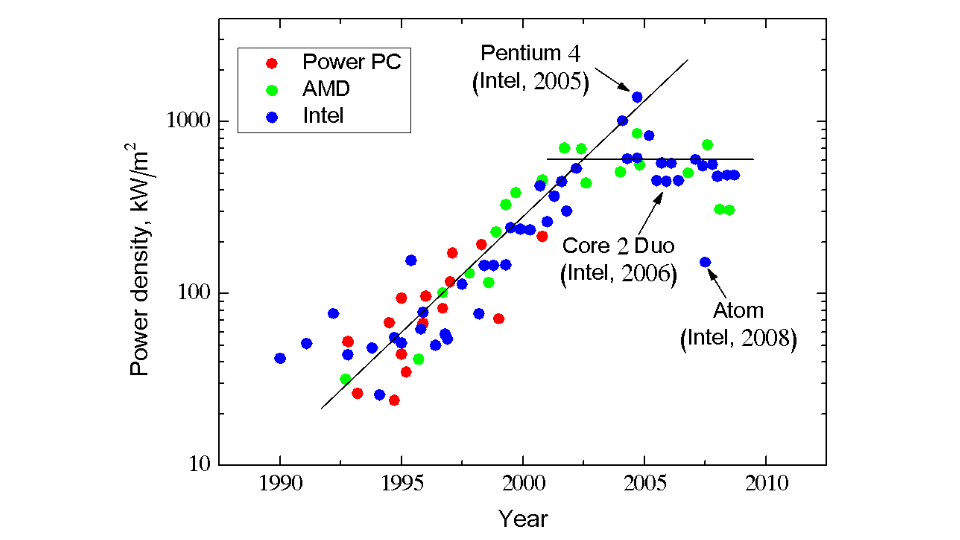
\includegraphics[width=13cm]{cpu_heat_flux.png}
  \caption{Power density of modern CPU \cite{okajima}}
  \label{fig:cpu}
\end{figure}

Most of today’s cooling devices are utilizing forced convection of air or liquid,
while boiling phenomena can evidently offer higher heat transfer coefficient, difficulty
in control flow boiling phenomena makes it to be seldom used in the normal electronic
product. Additionally, the normal scale boiling is dominated by nucleate boiling and
it is known that such cooling technique will fail if the heat flux exceeding critical
heat flux is generated from the device surface because of the “dry out” of heat transfer
surface.

In order to exceed this barrier and also improve the controllability, a cooling
technique utilizing evaporation of liquid film in a microchannel has been proposed by our
laboratory (at Tohoku Univ.). In a microchannel, as long as the nucleate boiling is
suppressed by controlling channel diameter, expansion of a single bubble and evaporation
of liquid film surrounding it will dominate the flow pattern.
Although two-phase flow in a microchannel has been
extensively studied in the last two decades, research focusing on the film behavior and
heat transfer characteristic is far from sufficient and a deeper understanding was needed
to develop such cooling devices.

The objectives of this study are to formulate a simulation
program and by simulating bubble fluid flow, to understand fluid flow and heat transfer
characteristic inside microchannel and help the development of innovative film evaporating
cooling technique.

\section{My approach for the project}

The original plan was to build my own two-phase flow solver from scratch.
The reason that we didn't consider a commercial software package (like ANSYS Fluent) or
opensource one (OpenFOAM) was:
\begin{itemize}
\item{Commercial software may lack the flexibility in terms of hackability since the core solver is
proprietary and no source code will be available for studying or modifying.}
\item{Available opensource code, for example OpenFOAM, has a massive code base and complex
class structure, which may make it too time consuming to study it thoroughly.}
\end{itemize}

As shown in Fig. \ref{fig:master_plan},there would be mainly 3 milestones in this approach:

\begin{itemize}
\item{Create an incompressible, single-phase, laminar flow solver.}
\item{Implemente interface tracking algorithm (VOF) \cite{Hirt1981201}.}
\item{Implemente surface tension model (CSF) \cite{Brackbill1992335}.}
\end{itemize}

\begin{figure}[h!]
  \centering
  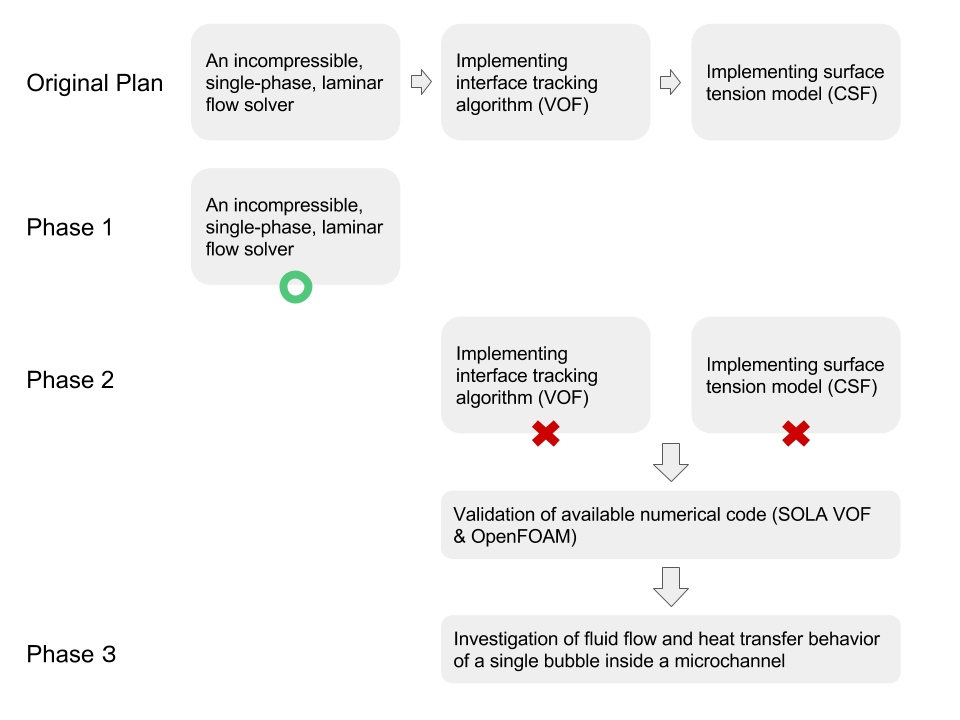
\includegraphics[width=15cm]{master_plan.png}
  \caption{A diagram explaining my master's degree research}
  \label{fig:master_plan}
\end{figure}

In the first year, a single-phase flow solver (implemented the
SIMPLE algorithm \cite{patankar1980numerical}), written in Matlab language was successfully developed.
However, when I tried
to implement the VOF method on top of my code, I noticed that the lack of
consideration over program structure and function/class interfaces in my design became a major obstacle
that prevent me from developing further complex algorithm.

On the other hand, thoroughly learning through those programming techniques was something I could not
afford as a master student. Thus in the second year, I changed the approach from building
everything from scratch to utilizing available numerical code.

Results of each phase of my research are described in the following sections.

\section{Phase 1: Creating a SIMPLE method simulator in Matlab from scratch}

In this phase, a simple solver for single-phase, laminar flow implementing the
SIMPLE algorithm was created from scratch (in Matlab). Navier-Stokes equations for incompressible
flow are selected to model the problem:

\begin{equation}
  \nabla \cdot \vec v = 0
\end{equation}
\begin{equation}
  \frac{\partial (\rho \vec v)}{\partial t} + \nabla \cdot (\rho \vec v \vec v) = - \nabla p +
  \mu \nabla^2 \vec v+ \rho g + F_b
\end{equation}
\begin{equation}
  \frac{\partial \rho c_p T}{\partial t} + \nabla \cdot (\rho c_p T \vec v) = \nabla \cdot \vec q
\end{equation}

\nomenclature{$\vec v$}{Flow velocity vector.}
\nomenclature{$\rho$}{Fluid density.}
\nomenclature{$p$}{Pressure.}
\nomenclature{$\mu$}{Dynamic viscosity.}
\nomenclature{$g$}{Gravity (vector).}
\nomenclature{$F_b$}{Other body forces.}
\nomenclature{$c_p$}{Specific heat of fluid.}
\nomenclature{$\vec q$}{External heat flux.}

Some preliminary simulations were carried out to prove the correctness of this computation code.
A typical piple flow model was built and tested as shown in Fig. \ref{fig:h-g_model}.
The velocity profile on the exit was compared with solution of a typical Hagen-Poiseuille flow case.

\begin{figure}[h!]
  \centering
  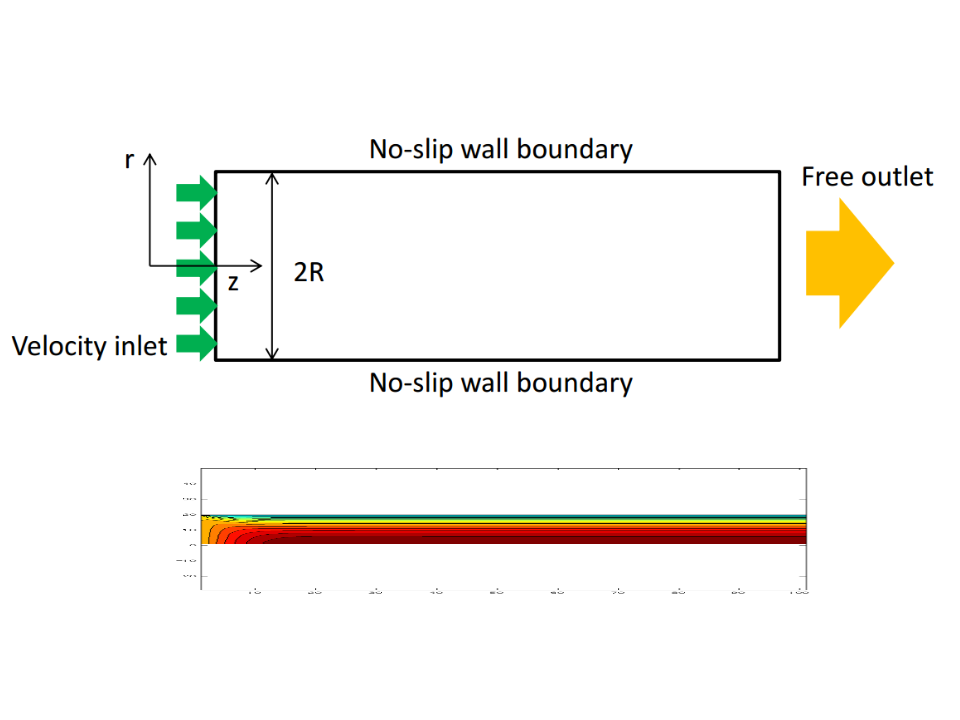
\includegraphics[width=13cm]{h-g_flow_model.png}
  \caption{A test case for validation}
  \label{fig:h-g_model}
\end{figure}

\begin{figure}[h!]
  \centering
  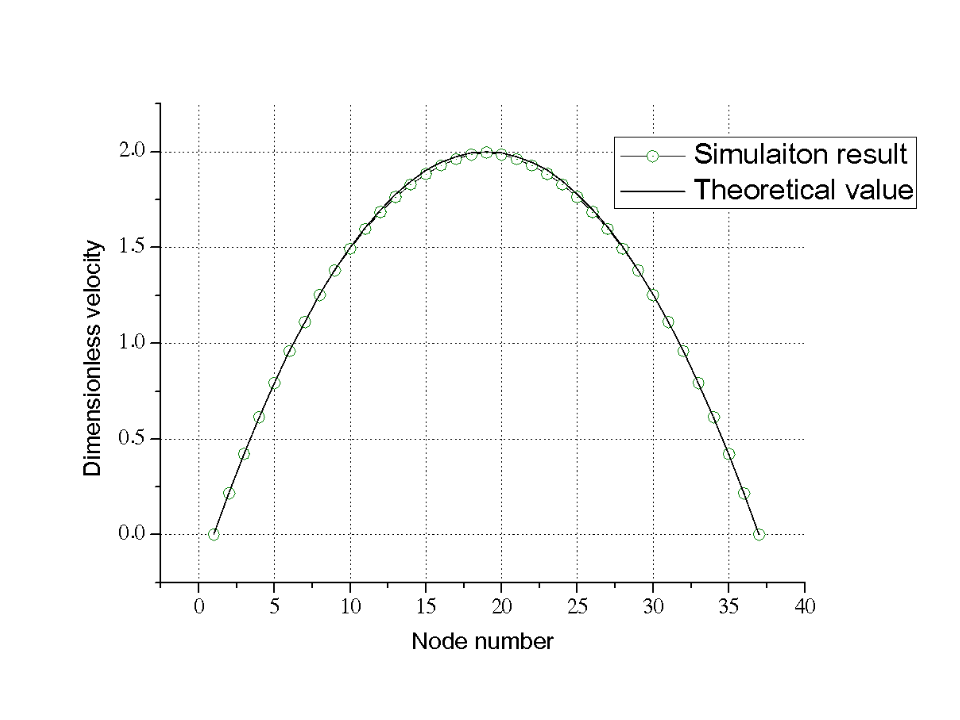
\includegraphics[width=12cm]{h-g_flow_result.png}
  \caption{Velocity profile on the exit of pipe flow model}
  \label{fig:h-g_result}
\end{figure}

I learned extensively about the SIMPLE method and observed how the velocity/pressure 
boundary conditions are related to each other. It was especially fascinating for me to observe
how the order of a matrix (invertible or not) affects the result of the iteration process.

%In addition, the resistance by sphere and cylinder was also calculated and showed
%well agreement with theoretical solution from Stokes flow.

\section{Phase 2: Validation of SOLA-VOF and further results}

As described before, in order to obtain reasonable simulation data of two-phase flow, I switched
to an available VOF solver called SOLA-VOF (in Fortran language).
SOLA-VOF is a numerical solver package for two-phase flow which was originally
developed at the Los Alamos National Lab in 1980s \cite{nichols1980sola}, and it became available
for academical use recently.

To test the ability of the solver, I conducted several numerical experiments including the
famous "dam break" (in Fig.\ref{fig:dam_break}) test case.
I also proposed a "steady bubble" test case to test the ability of the solver for micro bubble.
(in Fig.\ref{fig:steady_bubble}). 

In the "dam break" case, the calculated results showed good agreement with experimental
data\cite{dambreakexp}. 

\begin{figure}[h!]
  \centering
  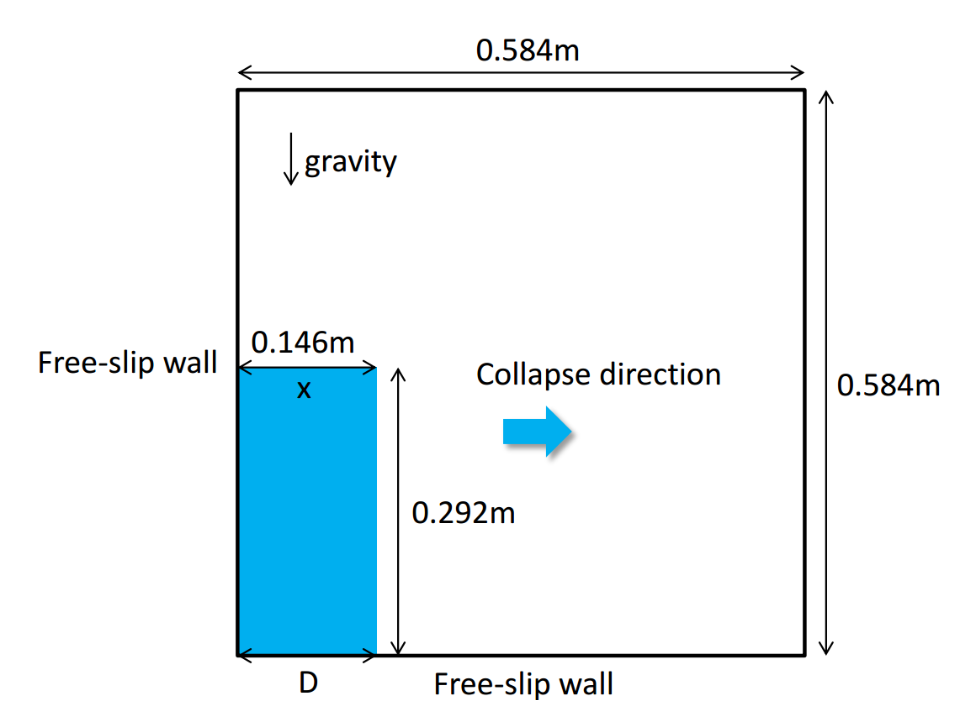
\includegraphics[width=11cm]{dam_break.png}
  \caption{A typical dam break test case}
  \label{fig:dam_break}
\end{figure}

In the "steady bubble" case, an air bubble is surrounded with water at a resting state.
No gravity or other body force is included so it's expected that no velocity in both
gas and liquid phase should occur. However, due to the surface tension model utilized in
SOLA-VOF has a nature to generate unreal numerical velocity \cite{Brackbill1992335}, it was
found that the interface was under unstable condition and the original bubble shape would be destroyed
under some conditions.

\begin{figure}[h!]
  \centering
  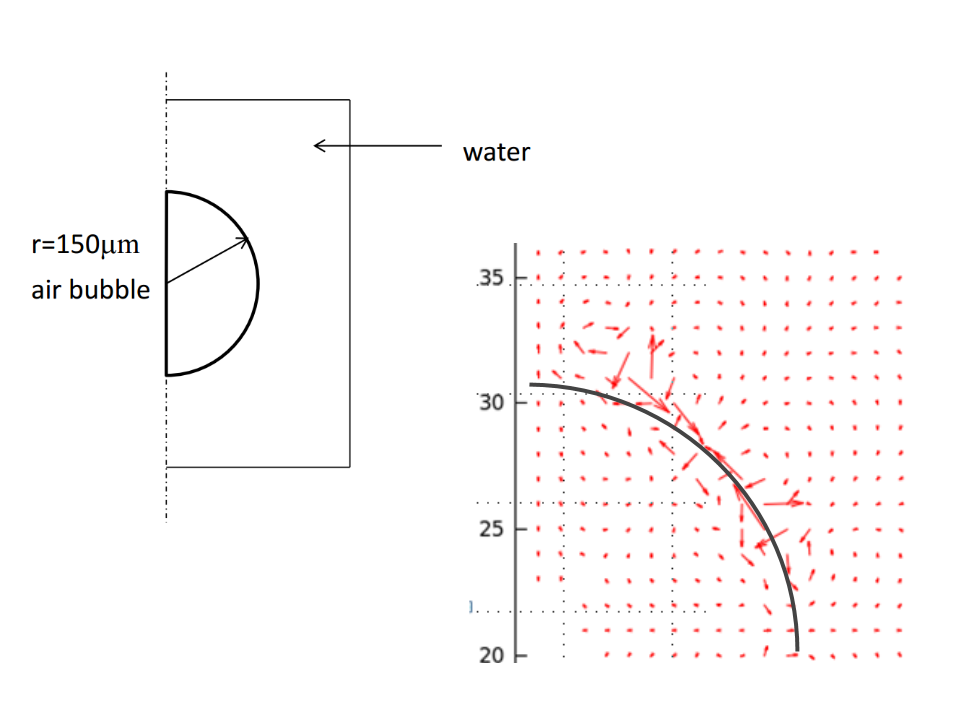
\includegraphics[width=12cm]{steady_bubble.png}
  \caption{A "steady bubble" test case and the parasitic current velocity observed}
  \label{fig:steady_bubble}
\end{figure}

Several numerical experiments were carefully conducted to
show the behavior of single bubble inside a microchannel.

Fig.\ref{fig:bubble_channel} shows the physical model and the results. The velocity of
gas phase (air) and liquid phase (water) at the inlet is $1 m/s$, and the diameter of the
channel is $280 \mu m$. The inlet velocity should be kept above certain value otherwise the
parasitic current velocity may dominate the flow pattern and thus the results would be
meaningless. It was also noted that due to the lack of grid resolution near the wall boundary,
there may occur numerical "dry out" in which the liquid film surrounding the bubble disappear
as if the liquid film is evaporated by heat.

\begin{figure}[h!]
  \centering
  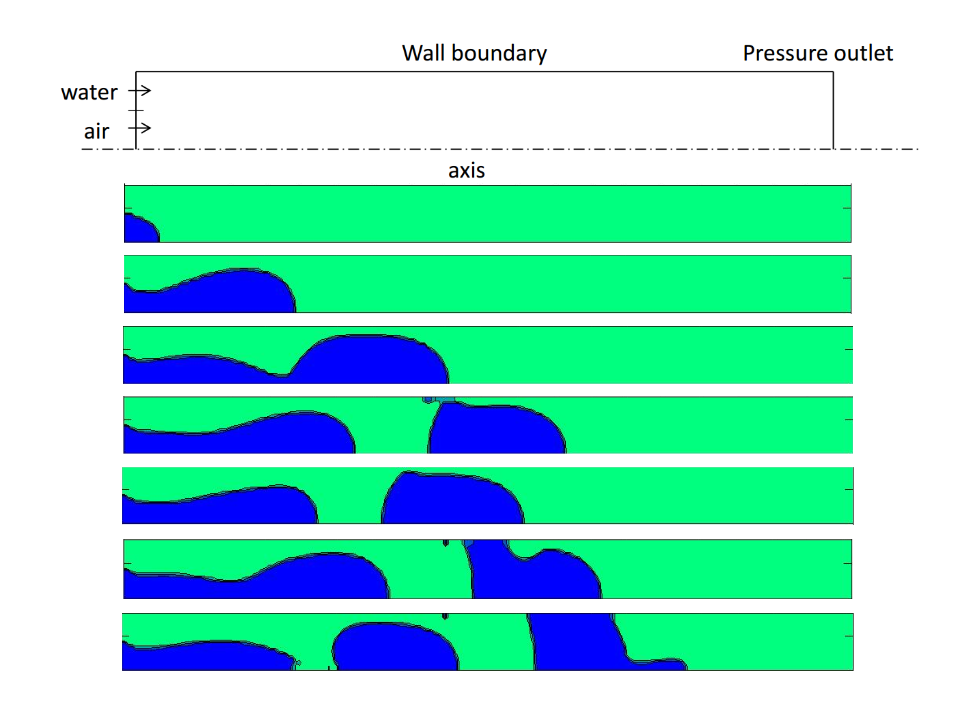
\includegraphics[width=12cm]{bubble_channel.png}
  \caption{A microchannel model and numerical results showing the bubble shape}
  \label{fig:bubble_channel}
\end{figure}

The bubble shape was compared with experimental result from other references\cite{Triplett1999377}
in Fig.\ref{fig:bubble_shape} and showed good agreement.

\begin{figure}[h!]
  \centering
  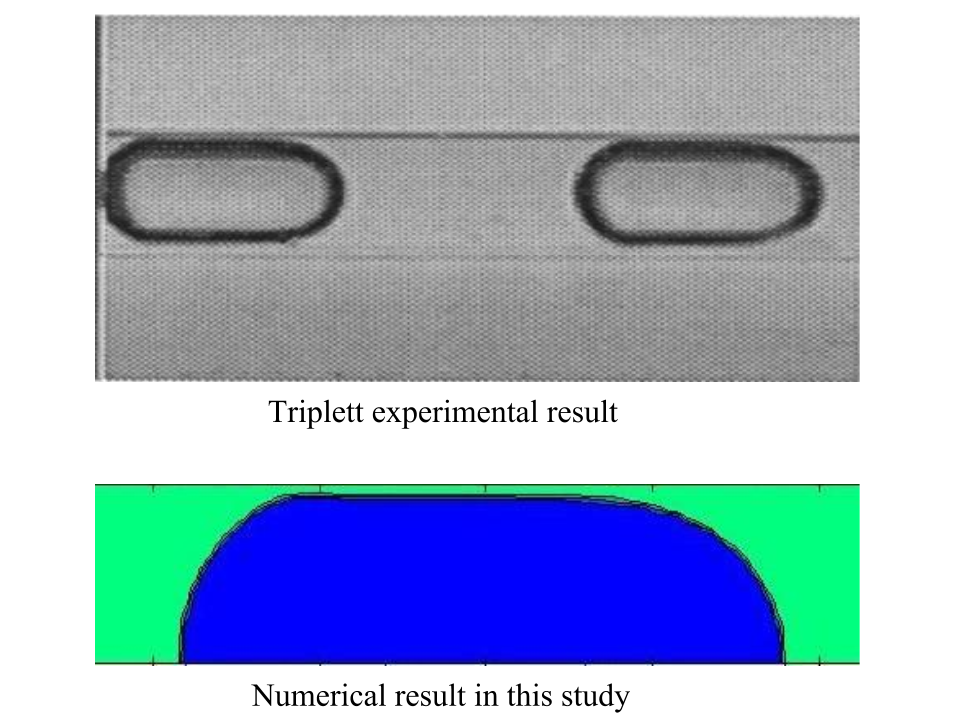
\includegraphics[width=10cm]{bubble_shape.png}
  \caption{Calculated bubble shape compared with experimental result}
  \label{fig:bubble_shape}
\end{figure}

As a final step, energy equation was added to the solver to calculate the temperature
distribution and heat exchange between the fluid and the wall. It should be mentioned that
no phase change model was included and as a result, the bubble could not grow or shrink
as what it's expected to behave in reality.

\begin{figure}[h!]
  \centering
  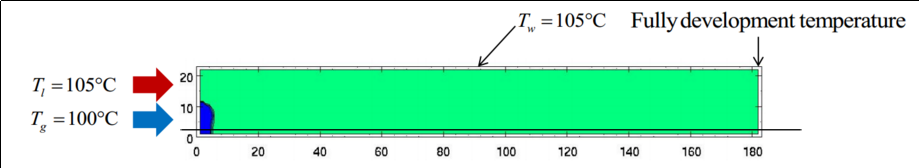
\includegraphics[width=15cm]{heat_model.png}
  \caption{Temperature boundary condition used in this study}
  \label{fig:heat_model}
\end{figure}

Fig.\ref{fig:heat_model} shows that the gas phase temperature was fixed on 100\celsius
 and the temperature of overheat water was 105\celsius. The wall temperature was also
fixed to 105\celsius  and thus heat would be absorbed from wall due to the existence
of thin liquid film between gas bubble and wall boundary.

\begin{figure}[h!]
  \centering
  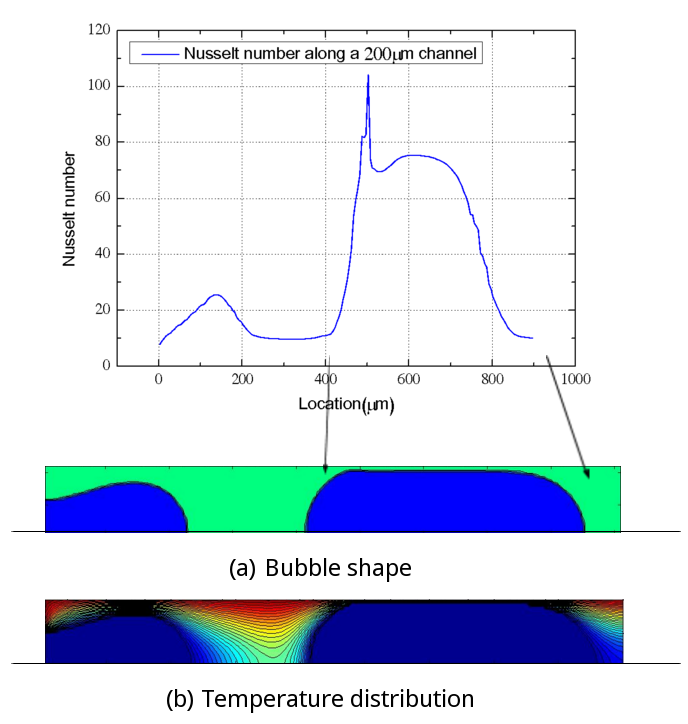
\includegraphics[width=12cm]{nusselt_result.png}
  \caption{Calculated temperature distribution and derived Nusselt number}
  \label{fig:nusselt_result}
\end{figure}

Fig.\ref{fig:nusselt_result} shows the calculated result of Nusselt number along the
long-axis of the channel. The Nusselt number was defined as below to reflect the
heat exchange rate:
\begin{equation}
Nu = \frac{q_w}{T_w-T_b} \frac{d}{k_L}
\end{equation}

\nomenclature{$Nu$}{Nusselt number.}
\nomenclature{$q_w$}{Heat flux on the microchannel wall.}
\nomenclature{$T_w$}{Wall temperature of a microchannel.}
\nomenclature{$T_b$}{Average temperature on cross section of a microchannel.}
\nomenclature{$d$}{Diameter of the microchannel.}
\nomenclature{$k_L$}{Heat conduction of the fluid.}

And $T_b$ is an artificial temperature used to represent the average temperature on
a cross section of the channel.

It was found that the existence of liquid film greatly promoted the heat exchange
between the fluid and wall, even there was no evaporation effect included in this
study. And the spike of Nusselt number on the tail of the bubble suggested that the
thickness of liquid film would be a key factor that affect the heat exchange rate.

\section{Concluding remarks}

The objectives of this study are to formulate a simulation program and by simulating
bubble fluid flow, to understand fluid flow and heat transfer characteristic inside
microchannel and help the development of innovative film evaporating cooling technique.

In the first phase of this study, I successfully built a single phase laminar flow
solver in Matlab. In order to validate the single-phase solver, velocity profile on exit was
compared with solution of Hagen-Poiseuille flow in pipe. Results showed good agreement
but due to the lack of experience in software development and limitation of time, I decided
to change the approach and utilize an available numerical code to continue the study.

In the second phase of this study, I studied the source code of SOLA-VOF method and validated
it by conducting several numerical experiments. Although some numerical issues including parasitic current
and numerical dry out near wall boundary was found, by carefully setting up the calculation
case, a single bubble flow inside a $280\mu m$ microchannel was successfully simulated.
Expansion and acceleration of bubble caused by the evaporation of liquid film was neglected
to simplify the phase change calculation procedure. Film thickness was found to be extremely
important which affects the heat flux directly. Nusselt number and the heat flux
result were used to evaluate the cooling ability in current simulation model.

As future work, numerical method to suppress the "parasitic current" will be necessary
since the existence of this unreal numerical velocity limited the computable velocity
range. Including the evaporation model will make it possible to simulate actual bubble
growth and shrink instead of air bubble, which will certainly increase the value of
the numerical results and may suggest interesting investigation for further experimental
research.


%Notes on how to compile references in bibtex:
%1. Compile main.tex by xelatex, this generate a bunch of .aux files
%2. Compile main.tex by biber, this generate main.bll and main.blg file
%3. Compile main.tex again by xelatex, now the reference should display at the end
%4. Compile main.tex with xelatex one more time...

%Extra note:
%Bibtex will sort the references in different order so use unsrt to override
%authors should all be connected with the word and, not comma

%\bibliographystyle{unsrt}
%\bibliography{sample}
%\printnomenclature

\clearpage
\printbibliography[title=References]

\clearpage
\printnomenclature

\end{document}
